\documentclass[UTF8]{ctexart}

\usepackage{subfiles}  

%下面的语句, 引入你的头部设置文件
\usepackage{C:/phpStorm_proj/02_myself_ID_EGO/+100_latex_all_math_sel/myPreamble} 
%必须是绝对路径, 才能让各个tex在单独编译时使用到

\title{物理}


%---------------------------------


\begin{document}
	\tableofcontents % 生成目录
	\date{} % 若不写这句, 则默认也会渲染出日期, 所以我们要手动赋空值
	\maketitle  %这行代码, 让你前面的 title, author, date生效
	
	

\vspace{1em} 

\subsection{加速度 $Acceleration=\frac{\varDelta v}{\varDelta t}$}

【加速度 Acceleration】:\\
假定一个质量为m的物体, 在光滑的水平面上, 受到恒力F的作用, 做匀速直线运动。在初始时刻, 物体的速度为v; 经过一段时间 Δt,它的速度为t',那么, 这个物体在这段时间的``加速度 Acceleration"就是: \\
\begin{align*}
	\boxed{
		\text{加速度}Acceleration=\frac{\varDelta v}{\varDelta t}=\frac{v'-v}{\varDelta t}		
	}
\end{align*}

\textbf{我们用``加速度"这个物理量, 来描述物体``速度变化快慢"的程度。如果物体的速度不变,那它的加速度等于 0 ;如果物体的速度在 1s 内, 从2m/s 增加到了 4m/s,那它的加速度就是 2m/s};如果物体的速度在2s 内, 从 1m/s 增加到了 7m/s,那么它的加速度就是:$\frac{(7-1)<m/s>}{2<s>}=3<m/s^2>$\\

加速度的单位, 一般是: 米/二次方秒. 符号是 $m/s^2$ 或 $m·s^{-2}$.\\



【加速度, 是矢量物理量, 是有方向的】:\\
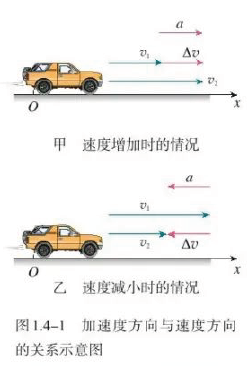
\includegraphics[width=0.4\textwidth]{img/0107.png}\\

如上图, 汽车原来的速度是v1,经过一小段时间 Δt后, 速度变为 v2。我们用一个新的有向线段Δv,来表示速度的变化量。 \\
由于加速度$a=\frac{\varDelta v}{\varDelta time}$,所以加速度a的方向, 与速度的变化量Δv 的方向相同。换言之, 确定了Δv 的方向, 也就确定了加速度a 的方向。\\

从图中可以看出:  \\
- 汽车在直线运动中,如果速度v 增加, 即加速运动, 则``加速度a" 的方向, 是与``初速度v1"的方向相同的. \\
- 如果速度减小,即减速运动, 则``加速度a"的方向, 是与``初速度v1"的方向相反的。\\

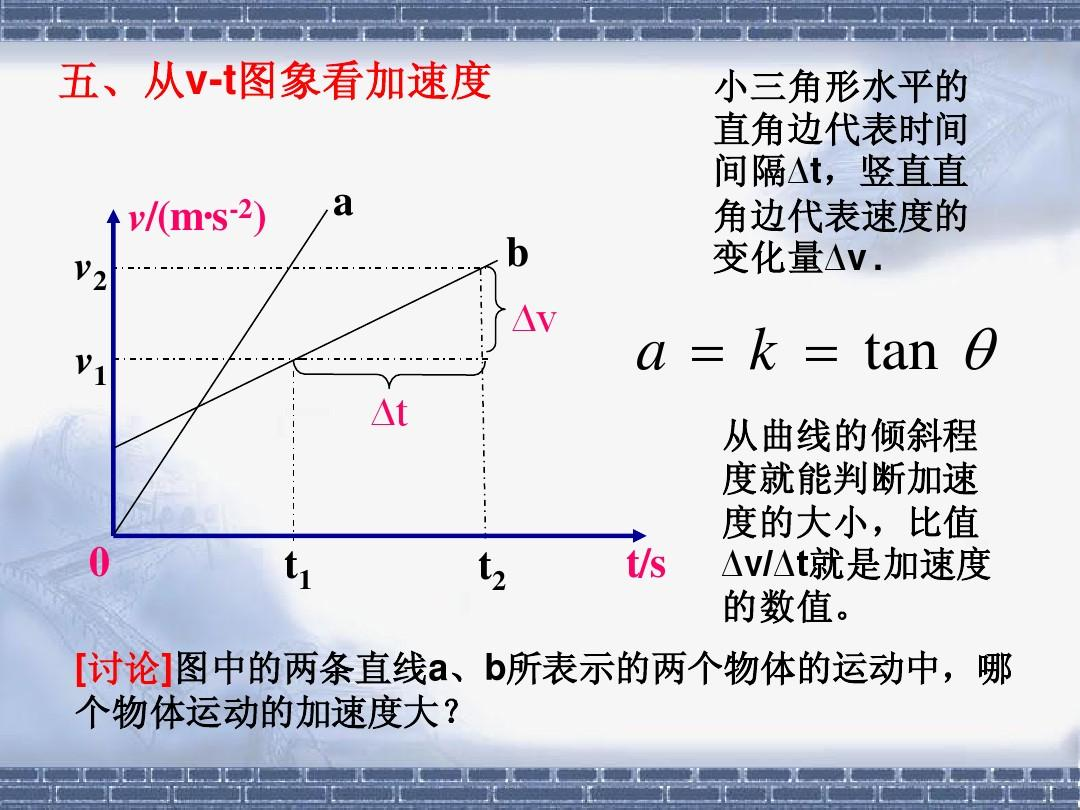
\includegraphics[width=0.5\textwidth]{img/0108.jpg}

	
	\vspace{1em} 
	
\subsection{变化率}

自然界中, 某量D的变化, 可以记为 ΔD. 发生这个变化所用的时间间隔, 可以记为Δt. 则 $\dfrac{\varDelta Data}{\varDelta time}$, 即ΔD与Δt的比值, 就是这个量对时间的``变化率".\\

某个量大,不代表它的变化率大。比如: \\
- 速度v 大的,加速度a 不一定大. 匀速飞行的高空侦察机,尽管它的速度可能接近 1000 m/s,但它的加速度为0。\\
- 速度v 小的,加速度a 也可以很大。例如枪筒里的子弹,在开始运动时,尽管子弹的速度接近0,但它的加速度可以达到 $5×10^4 m/s^2$.\\

\vspace{1em} 


\subsection{匀变速直线运动 : $v = v_0 + at$.}	

【匀变速直线运动  uniform variable rectilinear motion】: \\
即``加速度a" 不变的直线运动。意思是: 在任意相等的时间内, 速度的变化量 Δv 都相同. (加速度不变). ``匀变速直线运动"的v-t图像, 是一条倾斜的直线。\\	
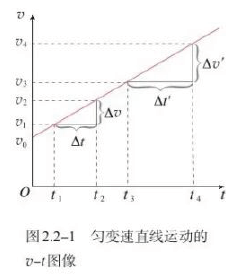
\includegraphics[width=0.4\textwidth]{img/0108.png}	\\
	
	
【匀加速直线运动】:\\
在``匀变速直线运动"中:\\
- 如果物体的速度, 随时间均匀增加,则这种运动叫作``匀加速直线运动". \\
- 如果物体的速度, 随时间均匀减小, 则这种运动叫作``匀减速直线运动". \\


【匀变速直线运动, 其两个参数 velocity(速度) 和 time 的关系公式就是】:\\
$	\text{加速度}a=\dfrac{\varDelta v}{\varDelta t}=\dfrac{\overset{\text{在}t\text{时刻的速度}}{\overbrace{v}}-\overset{\text{开始时刻的速度,即初速度}}{\overbrace{v_0}}}{\varDelta t}$ \\
即:
\begin{align*}
	\boxed{
		v=v_0+a\varDelta t
	}
\end{align*}
上面公式是什么意思呢?  \textbf{由于加速度a, 在数值上等于``单位时间内,速度的变化量", 所以 a×Δt 就是``Δt时间内,速度的变化量". 再加上运动开始时物体的速度 $v_0$, 就得到 ``t时刻物体的速度v".} \\



\begin{myEnvSample}
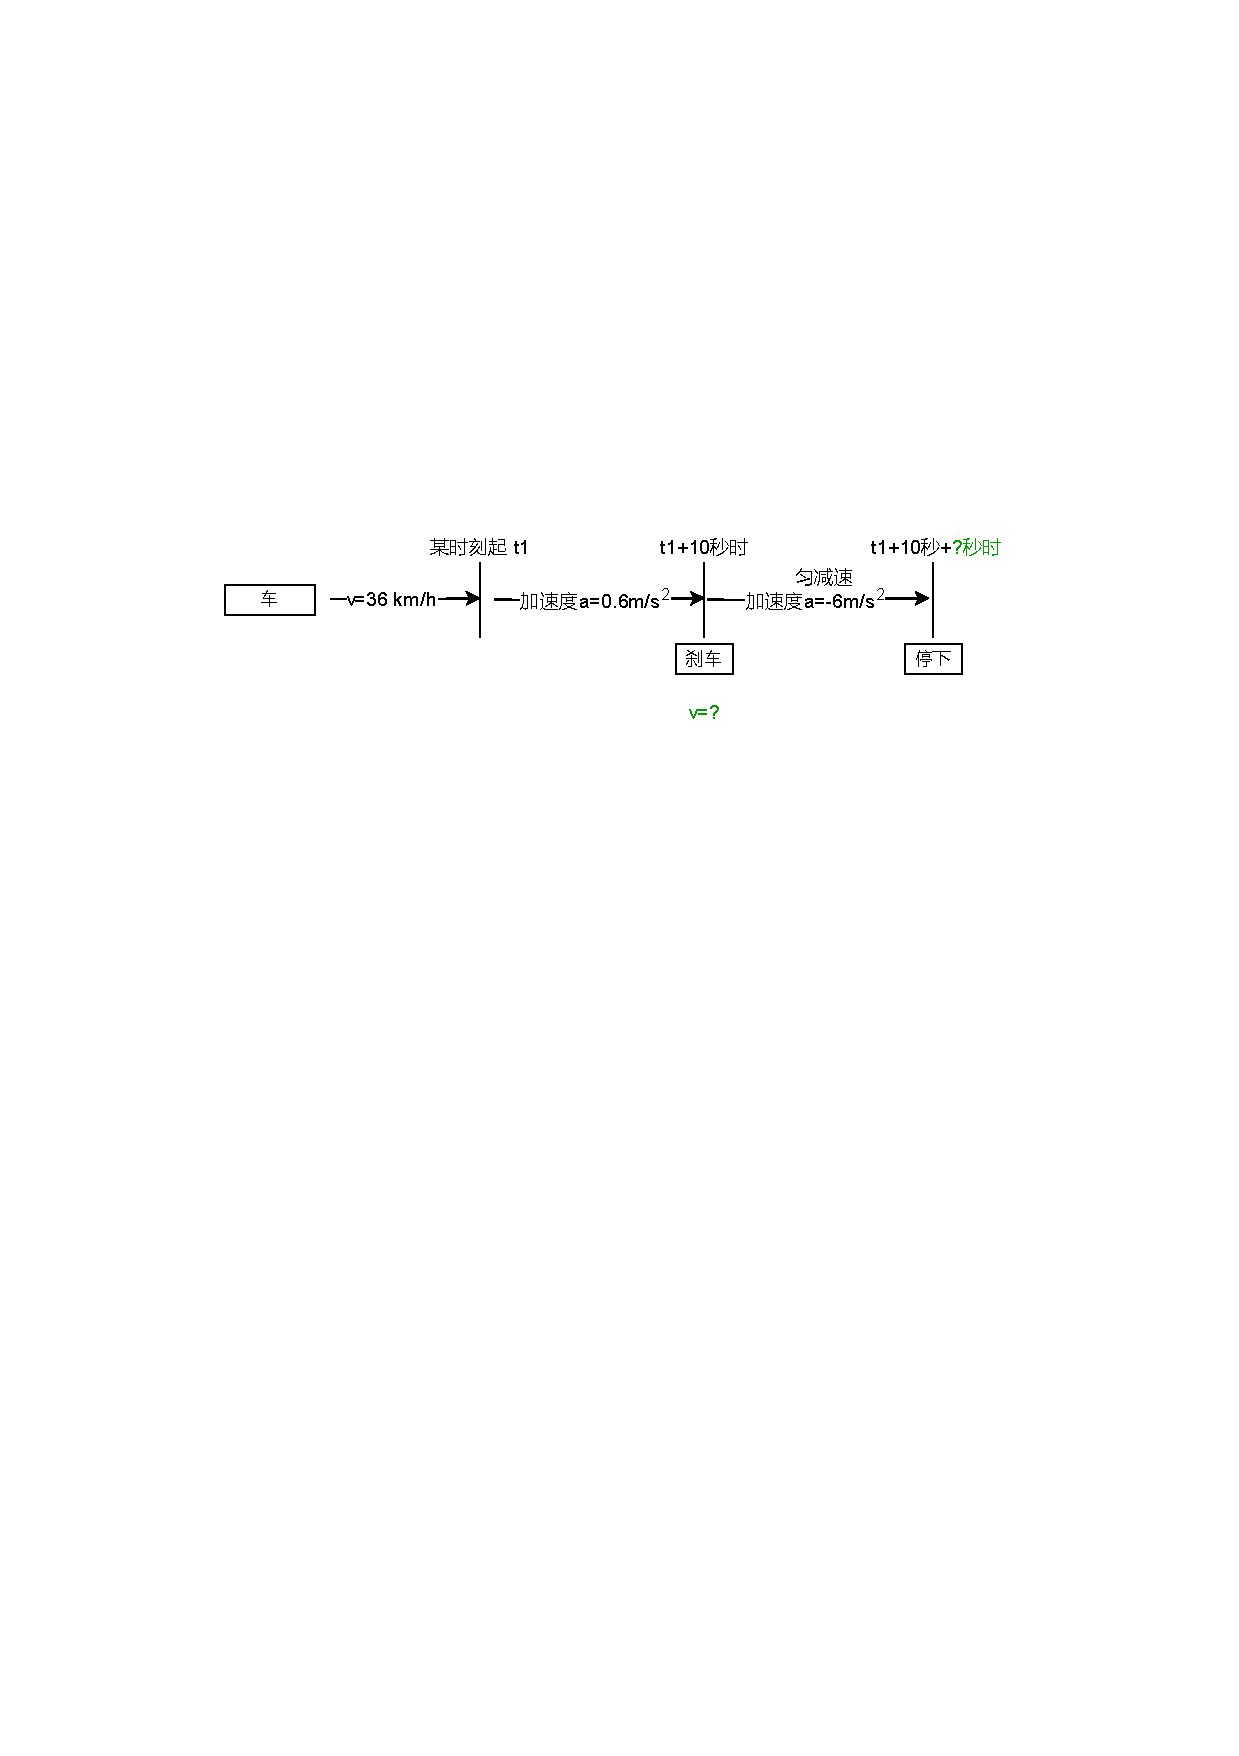
\includegraphics[width=1\textwidth]{img/0110.pdf}\\

一辆汽车以 36 km/h 的速度匀速行驶。从某时刻起, 它以 $0.6 m/s^2$ 的加速度加速,10 s末因故突然紧急刹车,刹车时做匀减速运动的加速度大小是 $6 m/s^2$, 直到汽车停了下来。 问: \\
(1)汽车在10s末的速度, 是多少? \\
(2)汽车从刹车到停下来, 用了多长时间? \\

汽车在加速和减速时, 都在做``匀变速直线运动"。所以, 根据公式: \\
(1) : \\
$
\underset{10\text{秒时的速度}}{\underbrace{v}}=\underset{36\ km/h}{\underbrace{v_0}}+\underset{0.6\ m/s^2}{\underbrace{a}}\underset{10s}{\cdot \underbrace{\varDelta t}}=16\ m/s
$ \\

(2) :
\begin{align*}
		& v=v_0+a\varDelta t,\ \text{即}\varDelta t=\frac{v-v_0}{a}\\
	& \underset{\text{从刹车到停下时的所用时间}}{\underbrace{\varDelta t}}=\frac{\overset{\text{停下时的速度}=0\ m/s}{\overbrace{v}}-\overset{\text{刹车时的速度}=16\ m/s}{\overbrace{v_0}}}{\underset{\text{加速度}=\ -6\ m/s^2}{\underbrace{a}}}=2.67\ s
\end{align*}
\end{myEnvSample}




\subsection{匀变速直线运动的位移 : $\text{位移}x=v_0t+\frac{at^2}{2}$}

做``匀变速直线运动"的物体, 其位移大小, 可以用下图中的梯形面积来表示 (其实就是``求积分"的概念). \\
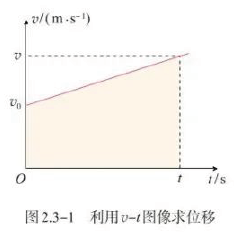
\includegraphics[width=0.3\textwidth]{img/0111.png} 
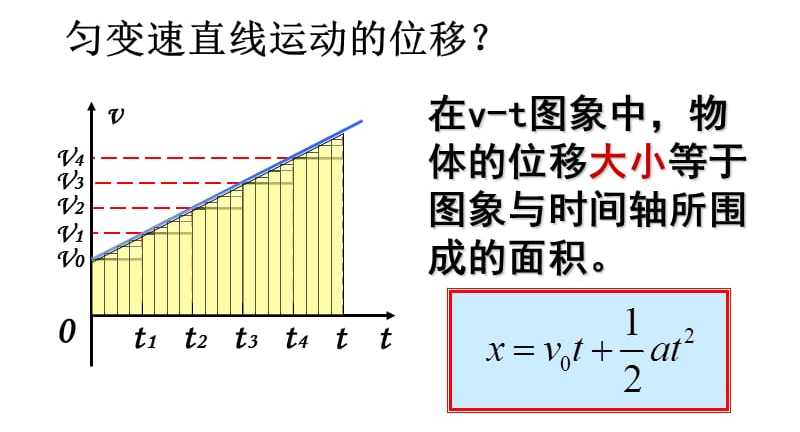
\includegraphics[width=0.5\textwidth]{img/0112.png} \\

所以, 位移x 就等于梯形的面积 = $\frac{1}{2}\left( v_0+v \right) t$\\
将 $v=v_0 + at$代入上式, 就有: \\
$
x=\dfrac{1}{2}\left( v_0+\underset{v=v_0+at}{\underbrace{v}} \right) t=\dfrac{1}{2}\left( 2v_0+at \right) t=\dfrac{2v_0t+at^2}{2}=v_0t+\dfrac{at^2}{2}
$ \\
即: 
\begin{align*}
	\boxed{
		\text{位移}x=v_0t+\frac{at^2}{2}
	}
\end{align*}

如果初速度$v_0$为0,这个公式就可以简化为: $\text{位移}x=\dfrac{at^2}{2}$\\


\begin{myEnvSample}

\end{myEnvSample}







	48
	
	
	
	
	
	
	
	
		
		
\section{动量p = 质量m × 速度v}

A球取碰撞B球, 碰撞后, A球停止运动而静止, B球开始运动, 最终摆到和A球拉起时同样的高度。 \\
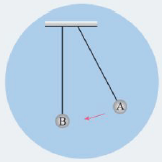
\includegraphics[width=0.2\textwidth]{img/0103.png} \\

对于发生碰撞的两个物体来说, 它们的 mv之和, 在碰撞前后可能是不变的。这使我们意识到: mv这个物理量具有特别的意义。
物理学中\textbf{把``质量m"和``速度v"的乘积mv, 定义为物体的``动量" momentum, 用字母p表示.} 
\begin{align*}
	\boxed{
\text{动量}p\ <kg·m/s>=\text{质量}m\cdot \text{速度}v
	}
\end{align*}

一般而言,\textbf{一个物体的``动量"指的是: 这个物体在它运动方向上保持运动的趋势。}\\

动量的单位, 是: 千克 米/秒, 符号是 kg·m/s. \\
\textbf{动量是矢量, ``动量的方向"与``速度的方向"相同.}\\


\begin{myEnvSample}
	一个质量为 0.1 kg 的钢球, 以 6m/s 的速度水平向右运动, 碰到坚硬的墙壁后弹回,沿着同一直线以 6 m/s 的速度水平向左运动。则碰撞前后钢球的动量变化了多少? \\

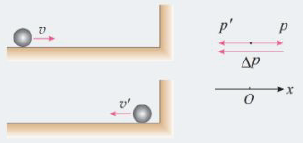
\includegraphics[width=0.4\textwidth]{img/0104.png} \\	

分析动量是矢量(矢量是既有``大小", 又有``方向"的物理量),虽然碰撞前后钢球速度的``大小"没有变化,但速度的``方向"变化了,所以动量的方向也发生了变化。所以为了求得钢球动量的变化量,需要先选定坐标轴的方向, 确定碰撞前后钢球的动量, 然后用碰撞后的动量, 减去碰撞前的动量, 就能求得动量的变化量。\\

我们就取水平向右, 为坐标轴的方向。则, 碰撞前的钢球的动量为: \\
$\text{动量}p=\text{质量}m\cdot \text{速度}v=0.1<kg>\cdot 6<m/s>=0.6<kg·m/s>	$ \\

碰撞后, 钢球的速度 v' = -6 m/s, 此时碰撞后钢球的动量为: \\
$\text{动量}p'=\text{质量}m\cdot \text{速度}v'=0.1<kg>\cdot (-6)<m/s>= -0.6<kg·m/s>	$ \\

所以, 碰撞前后钢球``动量"的变化量为: \\
$\varDelta p=p'-p=-0.6-0.6=-1.2<kg·m/s>$ \\

动量的变化量, 依然是矢量, 这里求得的数值为负值, 表示它的方向与坐标轴的方向相反, 即Δp的方向是水平向左。	
\end{myEnvSample}


所以一个物体受到的``合外力"越大,那它的速度就变化得越快,``加速度"就越大。 合外力,就是一个物体所受的所有外力的总和。 \\
物体的加速度, 还和该物体本身的``质量 m" 相关. 显然, 该物体的质量越大,同等``合外力"下获得的``加速度"就越小,反之就越大。所以,质量就成了一个衡量物体``运动状态改变难易程度"的物理量。质量越大,越重,就越不想动.\\
这样, 牛顿第二定律就呼之欲出了。\textbf{牛顿第二定律就是:物体的``加速度 a",  跟物体受到的``合外力 F" 成正比,跟物体的``质量 m" 成反比,写成公式就是 $\text{加速度}a=\frac{\text{合外力}F}{\text{质量}m}$.}, 即 $F=ma$. \\

\vspace{1em} 


\subsection{$\text{冲量}Impulse=\text{动量的变化值}\varDelta P=\text{合外力}F\cdot \varDelta time$}

进一步, 就有: 
\begin{align*}
		& \text{合外力}F=\text{质量}m\cdot \text{加速度}a\\
	& F=m\cdot \frac{\varDelta v}{\varDelta t}=m\frac{v’-v}{\varDelta t}=\frac{mv’-\overset{\text{即动量}p}{\overbrace{mv}}}{\varDelta t}=\frac{\overset{=\varDelta p}{\overbrace{p’-p}}}{\varDelta t}\\
	& \text{即:}\underset{\text{合外力}}{\underbrace{F}}\cdot \varDelta t=\underset{\text{动量的变化量}}{\underbrace{\varDelta p}}
\end{align*}

这个公式: $\underset{\text{合外力}}{\underbrace{F}}\cdot \varDelta t=\underset{\text{动量的变化值}}{\underbrace{\varDelta p}}$, 等号左边的值, 既与力F的大小、方向有关, 又与力的作用时间t有关。 等号右边的值 Δp, 是物体在 Δt这段时间内, ``动量"的变化量. \\
$FΔt$这个物理量, 就是``力"与``力的作用时间"的乘积, 该物理量有个名字, 叫``冲量" impulse. 取首字母I来表示冲量. 即:  \\
\begin{align*}
	\boxed{
	\underset{\text{合外力}}{\underbrace{F}}\cdot \varDelta t=\underset{\text{动量的变化值}}{\underbrace{\varDelta p}}=\text{冲量}I	
	}
\end{align*}

在经典力学里,\textbf{物体所受``合外力F"的``冲量 impulse", 等于它的``动量的增量 Δp"(即``末动量"减去``初动量"),叫做``动量定理".}\\
即:物体在一个过程中所受力的``冲量", 等于它在这个过程始末的``动量变化量"。这个关系叫作``动量定理" theorem of momentum.

\textbf{一个恒力的``冲量", 指的是``这个力"与其``作用时间"的乘积。}

冲量的单位是``牛秒", 符号是 N·S. \\

\textbf{物体在碰撞过程中, 受到的作用力, 往往不是恒力,物体不做匀变速运动。怎么处理这个问题呢? 就是用``微积分"的方法: 我们可以把碰撞过程, 细分为很多短暂过程(图1.2-2), 这样, 每个短暂过程中物体所受的力, 就没有很大的变化,这样对于每个短暂过程就能够应用 算出Δp了。然后把所有这些 Δp 相加, 就得到整个过程的动量定理。} \\

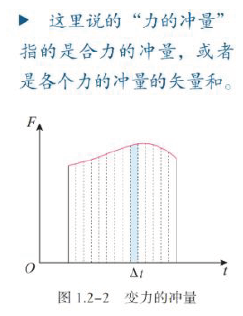
\includegraphics[width=0.3\textwidth]{img/0105.png}\\

注意: 此时, 在应用 $I= \Delta p = F \cdot \Delta t$  处理变力问题时, 式中的F应该理解为变``力在作用时间内的平均值"。 \\

根据动量定理公式: $\text{冲量}I= \Delta p = F \cdot \Delta t$, 可以知道: 如果物体的``动量p"发生的变化是一定的,那么: \\
→ 作用的时间t 短,物体受的力F 就大 \\
→ 作用的时间t 长, 物体受的力F 就小. \\

\begin{myEnvSample}
玻璃杯落在坚硬的地面上会破碎, 落在地毯上则不会碎, 用上面的``动量定理公式"解释就是: 虽然玻璃杯下落, 两种情况下的动量变化量 Δp 相等, 即冲量 I 相等. 但是: \\
- 杯子对地面的作用时间短, 所受的力 $F=\frac{\varDelta P}{\varDelta time}$ 就大. (分母越小, 分数值就越大) \\
- 杯子对地毯的作用时间长(因为有弹性缓冲), 所受的力 $F=\frac{\varDelta P}{\varDelta time}$ 就小. (分母越大, 分数值就越小) 
\end{myEnvSample}


\begin{myEnvSample}
一个垒球, 质量m=0.18kg, 以 25m/s的速度飞向球棒. 球棒与垒球的作用时间若为0.002s, 然后垒球反向水平飞回. 飞回时的速度为 45m/s. 问: 球棒对垒球的平均作用力, 是多大? \\
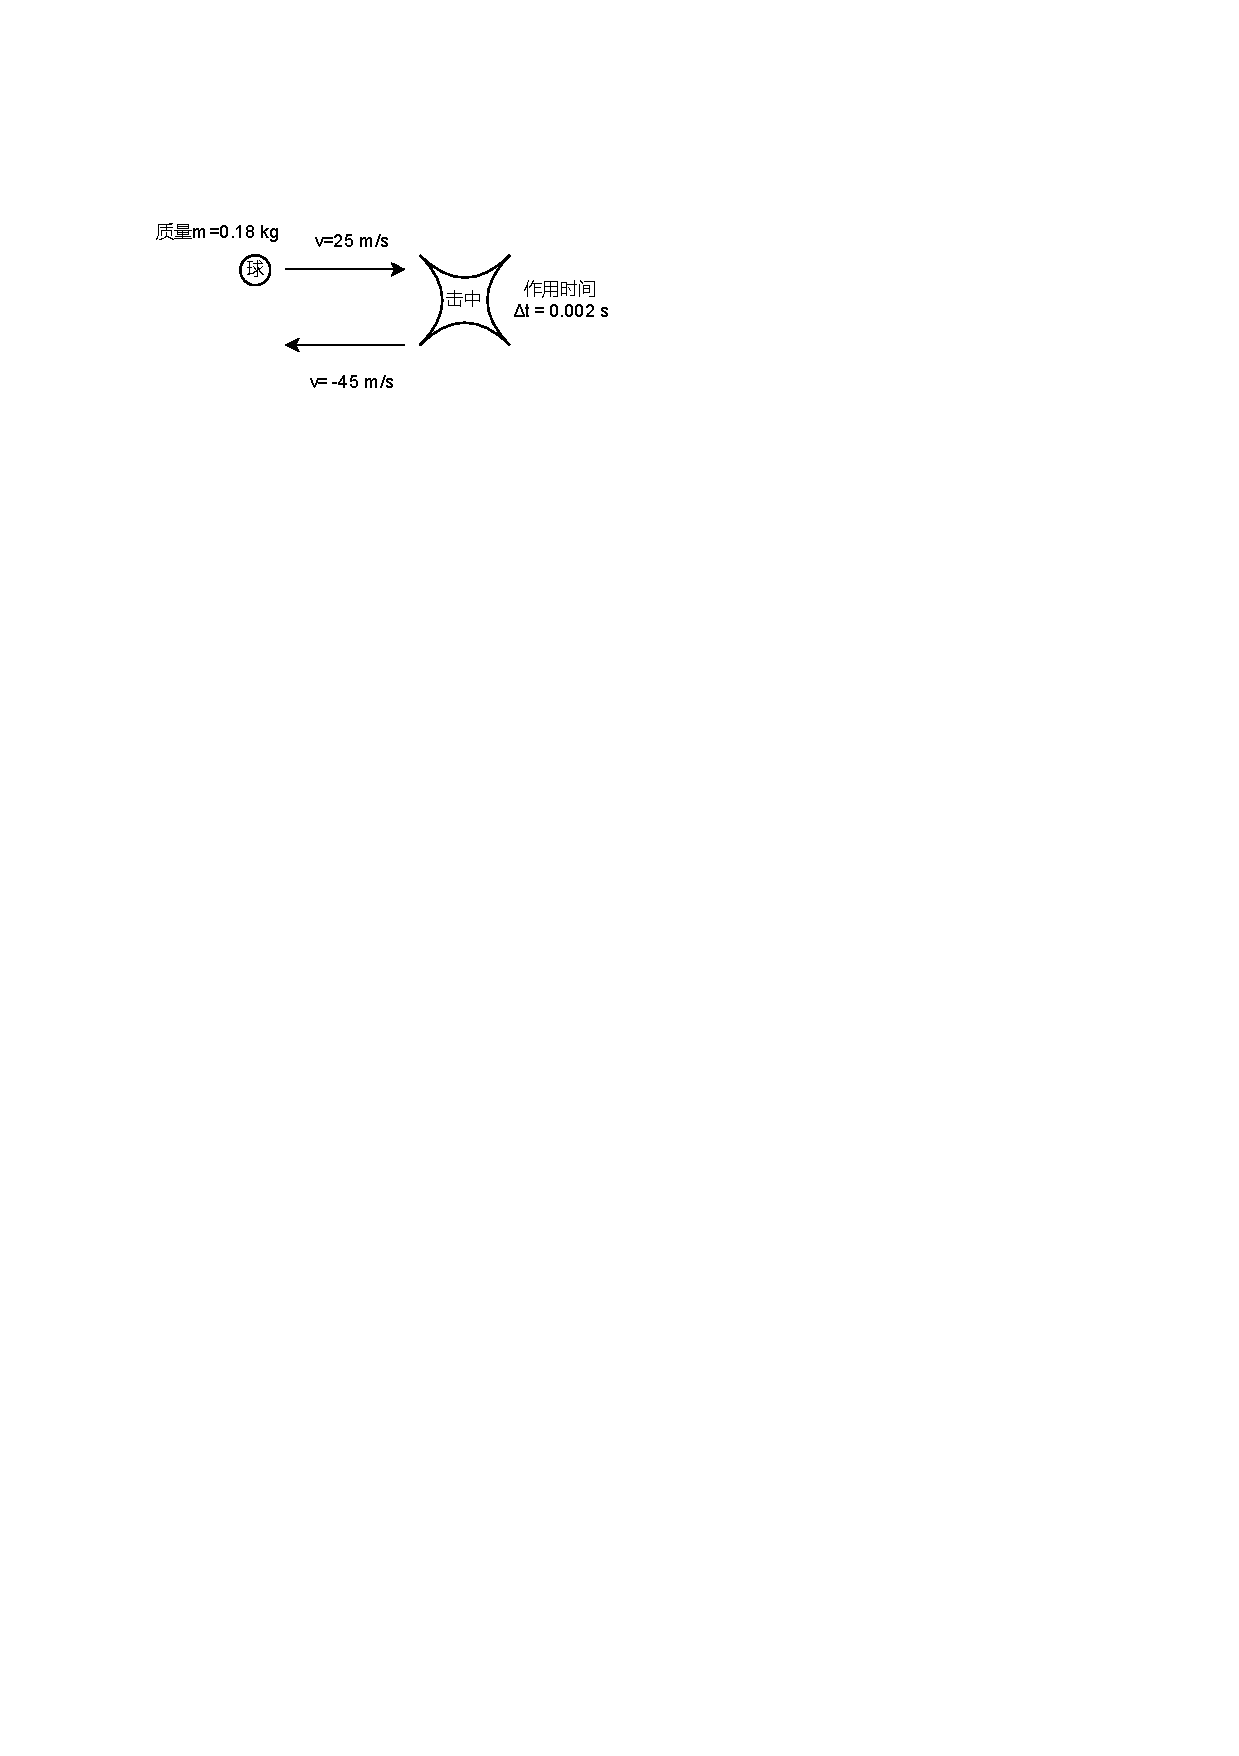
\includegraphics[width=0.5\textwidth]{img/0106.pdf} 
\begin{align*}
		&\text{垒球的初动量}p=mv=0.18<kg>\cdot 25<m/s>=4.5\ <kg·m/s>\\
	&\text{垒球的末动量}p=mv=0.18<kg>\cdot (-45<m/s>)=-8.1\ <kg·m/s>\\
	&\text{根据动量定理:\ }F=\frac{\varDelta p}{\varDelta t}=\frac{-8.1-4.5\ <kg·m/s>}{0.002\ s}=-6300N	
\end{align*}
上面, 若以垒球飞向球棒时的方向, 为坐标轴的正方向. 则垒球反向飞回时的方向, 就是坐标轴的负方向了, 所以要写上负号.
\end{myEnvSample}


力, 既可以通过``动量"来表示: $F=\dfrac{\varDelta p}{\varDelta t} $, \\
也可以用``动能"来表示: $F=\dfrac{\varDelta E_k}{\varDelta x}$ \\

→ \textbf{动量p, 决定了物体在力F 的阻碍下, 能够运动多长时间.} \\
→\textbf{ 动能E, 则决定了物体在力F 的阻碍下, 能运动多长距离。}\\
也就是说: \\
→\textbf{``动量定理"$I=\varDelta p=F\cdot \varDelta t$, 反映了``力对时间"的累积效应.} \\
→ \textbf{动能定理"$E_k=\frac{1}{2}mv^2$, 反映了``力对空间"的累积效应.} \\


\vspace{1em} 


\subsection{动量守恒定律}














14



		
		
	
	
\end{document}